% Copyright 2005-2016 Airbus-EDF-IMACS-Phimeca
% Permission is granted to copy, distribute and/or modify this document
% under the terms of the GNU Free Documentation License, Version 1.2
% or any later version published by the Free Software Foundation;
% with no Invariant Sections, no Front-Cover Texts, and no Back-Cover
% Texts.  A copy of the license is included in the section entitled "GNU
% Free Documentation License".
\renewcommand{\filename}{docUC_StocProc_MonteCarlo.tex}
\renewcommand{\filetitle}{UC : Monte Carlo Probability of an event based on a process}

% \HeaderNNIILevel
% \HeaderIILevel
\HeaderIIILevel

\label{MonteCarloProcess}

\index{Stochastic Process!Monte Carlo  based on process}



The objective of this Use Case is to evaluate the probability of an event based on  a stochastic process, using the Monte Carlo estimator.\\


Let $X: \Omega \times \cD \rightarrow \Rset^d$ be a stochastic process of dimension $d$, where $\cD \in \Rset^n$ is discretized on the mesh $\cM$.

We define the event $\cE$ as:
\begin{align}\label{eventProcStoch}
  \displaystyle \cE(X) = \bigcup_{\vect{t}\in \cM}\left\{X_{\vect{t}}  \in \cA  \right\}
\end{align}
where $\cA$ is a domain of $\Rset^d$. \\

We estimate the probabilty $p=\Prob{\cE(X)}$ with the Monte Carlo estimator.\\

The Monte Carlo algorithm is manipulated the same way as in the case where the event is based on a random variable independent of time. Details on the manipulation of the Monte Carlo algorithm and its results are presented in the Use Case  \ref{simuRes}. \\


\requirements{

  \begin{description}
  \item[$\bullet$] the domain $\cA$: {\itshape myDomainA}
  \item[type:] Domain
  \end{description}

  \begin{description}
  \item[$\bullet$] the process $X$: {\itshape myProcess}
  \item[type:] Process
  \end{description}
}
{
  \begin{description}
  \item[$\bullet$] the event $\cE$ : {\itshape myEvent}
  \item[type:] Event
  \end{description}

  \begin{description}
  \item[$\bullet$] the Monte-Carlo algorithm : {\itshape myMonteCarloAlgo}
  \item[type:] MonteCarlo
  \end{description}
}

\textspace\\
Python script for this Use Case :

\inputscript{script_docUC_StocProc_MonteCarlo}

\textspace\\

We illustrate the algorithm on the example  of the  bidimensionnal white noise process $\varepsilon: \Omega \times \cD \rightarrow \Rset^2$ where $\cD\in \Rset$, distributed according to the bidimensionnal standard normal distribution (with zero mean, unit variance  and independent marginals).\\
We consider the domain  $\cA =  [1,2] \times [1,2]$. Then the event $\cE$ writes :
\begin{align*}
  \displaystyle \cE(\varepsilon) = \bigcup_{\vect{t}\in \cM}\left\{\varepsilon_{t}  \in \cA  \right\}
\end{align*}
For all time stamps $t \in \cM$, the probability $p_1$ that the process enters into the domain $\cA$ at time $t$ writes, using the independence property of the marginals :
\begin{align*}
  p_1 = \Prob{\varepsilon_t  \in \cA} = (\Phi(2) - \Phi(1))^2
\end{align*}
with $\Phi$ the cumulative distribution function of the scalar standard \textit{Normal} distribution.\\
As the proces is discretized on a time grid of size $N$ and using the independance property of the white noise between two different time stamps and the fact that the white noise follows the same distribution at each time $t$, the final probability $p$  writes :
\begin{equation}\label{pexact}
  p = \Prob{\cE(\varepsilon)} = 1 - (1 - p_1)^{N}
\end{equation}
With $K=10^4$ realizations, using the Monte Carlo estimator, we obtain $p_K = 0.1627$, to be compared to the exact value $p=0.17008$ for a time grid of size $N=10$.\\

The Figure (\ref{mc_eventprocess_convergency}) draws the convergence graph of the estimator, with confidence level = $95\%$, equal to $CI_{0.95}= [0.168, 0.173]$.\\

\begin{figure}[H]
  \begin{center}
    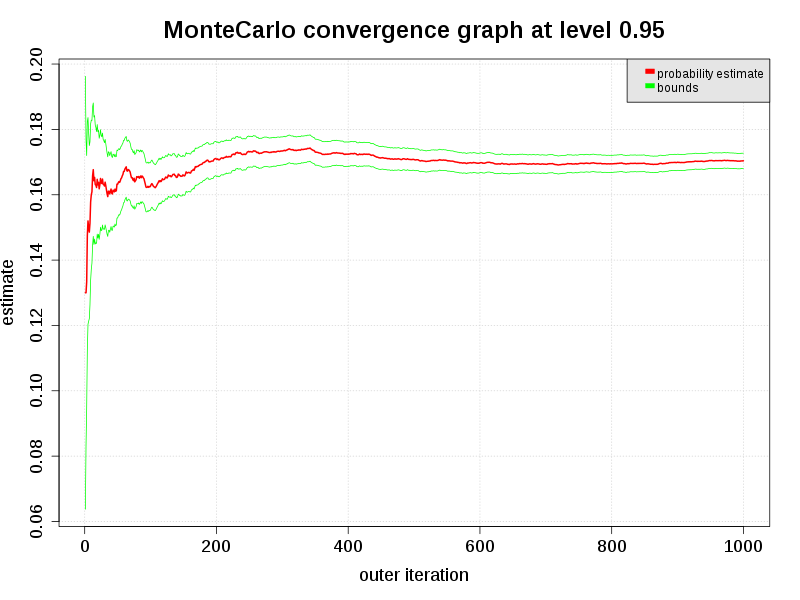
\includegraphics[width=7cm]{Figures/MonteCarloEventProcessConvergency.png}
    \caption{Convergence of the Monte-Carlo estimator based on a process event.}
    \label{mc_eventprocess_convergency}
  \end{center}
\end{figure}
